%! Author = Vova
%! Date = 28.07.2021

% Preamble
\documentclass[11pt]{article}

% Packages
\usepackage{amsmath}
\usepackage{hyperref}
\usepackage{polyglossia}
\usepackage{graphicx}
\usepackage{babel,blindtext}
\usepackage{subfig}
\usepackage{iftex}
\usepackage{xcolor}
\usepackage{amssymb}
\usepackage{adjustbox}
\usepackage[normalem]{ulem}
\usepackage{amsfonts}
\usepackage{placeins}
\usepackage{listings}

\lstset{basicstyle=\ttfamily,keywordstyle=\underbar,morekeywords={plot,solve,optimize,for,in,minorant}}

% Language and Font settings

% Kurale
% New Standard Old
\setdefaultlanguage{russian}
\setmainfont[Ligatures=TeX]{Kurale}
\newfontfamily\cyrillicfont{Kurale}

% Author, date
\title{Описание Математического Бота}
\author{Латыпов Владимир Витальевич}
\date{\today}

% Graphics settings
\graphicspath{{../images/}}



% Document
\begin{document}

    \maketitle
    \newpage

    \tableofcontents
    \newpage


    \section{Формулировка задачи}\label{sec:formulating-task}
    Математический бот — это набор инструментов для работы с математическими сущностями через интерфейс привычных нам социальных сетей.
    В отличие от WolframAlpha, бот специализируется на оптимизации многомерных функций и численном решении уравнений с большим количеством переменных
    (проверено, что с этим бот справляется лучше).

    Технически бот состоит из двух частей:
    \begin{itemize}
        \item Условный «front-end» — программа (написана на python), которая через vk\_api выполняет коммуникативную функцию, то есть общается с пользователем и,
        когда требуется, вызывает основной блок.
        \item А именно — «back-end» интерфейс, который написан на C++ и компилируется в полноценное консольное приложение.
        Он и занимается оптимизацией функций, решениями уравнений и т.д.
    \end{itemize}

    Поэтому больший интерес, конечно, представляет back-end часть.

    \section{Обзор}\label{sec:overview}

    Бот умеет:
    \begin{itemize}
        \item Оптимизировать функции
        \item Решать уравнения
        \item Строить графики
    \end{itemize}

    Третий режим добавлен для удобства — чтобы рассматривать функции (правда, пока только 2-х мерные),
    не выходя из диалога с ботом.

    Во всех случаях вводится математическое выражение и, возможно, дополнительные параметры.
    Предусмотренно два варианта введения запросов боту:
    \begin{itemize}
        \item Через коммуникацию: от пользователя требуется читать сообщения бота, предложенные ответы, знакомясь с интерфейсом бота,
              и, отвечать на них (зачастую достаточно выбрать вариант из предложенных).
              Этот вариант подходит для людей, которые только знакомятся с возможностями бота.
        \item Quick Input Mode (QIM).
              Если пользователь точно знает, что ему нужно и что значат аргументы, для него целесообразно использовать эту возможность.
              Вся информация для запроса передаётся одним сообщением, содержащим корректрую команду QIM.

        Типичный запрос выглядит так (переносы строки не важны): \newline

        \begin{lstlisting}[label={lst:QIM-example}]
            optimize x + y^2 - 1000.5
            for x in [-10; 100],
            y in (10.3e-100, 123)
            | minorant 10
        \end{lstlisting}

    \end{itemize}

    Подробнее об интерфейсе можно прочитать в Инструкции (ВСТАВИТЬ ССЫЛКУ!).


    В отличие от других подобных инструментов, бот предоставляет дружелюбный интерфейс: если пользователь что-то некорректно указал,
    бот известит его об этом.
    Однако иногда бот проверяет характер: например, ему не очень нравится, когда много раз неправильно указывают аргумент или
    когда пишут с маленькой буквы.

    \section{Технические подробности}


    \section{Описание алгоритма в общих чертах}

    \subsection{Разбор выражений}

    Оптимизация: если какая-то ветка полностью вычислима заранее (без знания переменных), она считается сразу.
    Если +0 или *1, это тоже убирается.


    \subsection{Дерево алгоритмов оптимизации}\label{subsec:opt-algo-tree}

    \subsubsection{Идея}
    Комбинируя разные алгоритмы, можно получить существенно более хороший результат, чем при запуске их по отдельности.
    Но важно понимать, в какой последовательности их лучше запускать.

    Здесь нужно понимать, что, проектируя алгоритм оптимизации, приходится выбирать между скоростью
    сходимости и вероятностью попасть в локальный оптимум, не найдя то, что искали (конечно, это упрощённая картина, но полезно посмотреть под таким углом).

    \begin{figure}[h]
        \centering
        
\includegraphics[width=0.6\textwidth]{balance.jpg}
        \label{fig:perfect-balance}
    \end{figure}
    \FloatBarrier

    Умение избегать локальных оптимумов ради нахождения глобальных назовём \underline{глобальностью} алгоритма.

    Для понимания, как комбинировать алгоритмы, полезна идея: когда алгоритм с высокой глобальностью уже нашёл некую окрестность, в которой,
    по его мнению, находится оптимум, имеет смысл передать его результат в более локальный алгоритм,
    чтобы увеличить скорость и точность без потери этой окрестности.

    Реализованные алгоритмы, которые могут быть полезны:
    \begin{itemize}
        \item Генетический алгоритм
        \item Алгоритм симуляции отжига
        \item Градиентный спуск
        \item Метод Ньютона
    \end{itemize}

    Алгоритмы расположены в порядке увеличения скорости сходимости и уменьшения глобальности.
    (Метод Ньютона можно назвать менее глобальным, чем градиентный спуск, так как он ищет не «ближайший» минимум,
    а любой «ближайший» экстремум (корень производной в данном случае))

    Причём у некоторых алгоритмов есть разные гиперпараметры, которые также регулируют этот скорость сходимости.
    Проанализировав всё это, я пришёл к выводу, что целесообразно подключение алгоритмов друг к другу примерно так, как это описано
    в следующем разделе.

    \subsubsection{Распределение вычислительного ресурса}\label{subsubsec:resource-distribution}

    В случае МатБота результаты профайлинга подтверждают предположение о том, что бо́льшая часть вычислительного времени ($\gg 95\%$)
    используется именно для подсчёта функции ошибки, а не для операций с геномами.

    В условиях, когда выделенное количество вычислительных ресурсов может быть разным для разных людей и запросов,
    особенно остро встаёт вопрос о распределении этих вычислительных ресурсов.


    \subsubsection{Схема дерева}

    \begin{figure}[h]
        \centering
        \adjincludegraphics[width=\textwidth, clip, trim={0.0\width} {0.35\height} {0.0\width} {0.0\height}]{OptTree_scheme.pdf}
        \caption{Схема дерева оптимизации}
        \label{fig:opt-tree}
    \end{figure}
    \FloatBarrier


    \section{Модификации в ГА}\label{sec:ga-modifications}
    Подробное описание ГА (в том числе — моей версии) можно найти в описании робота-художника в соответствующей секции.
    Здесь сосредоточусь на том, что относится конкретно к боту.

    В секции~\ref{subsubsec:resource-distribution} описано, как вычислительный ресурс распределяется между разными алгоритмами.
    Однако на том моменте, когда стало известно количество раз, сколько можно вычислить функцию ошибки вов время исполнения ГА,
    вопрос ещё не закрыт.

    Как известно, генетический алгоритм в каждую из $E$ «эпох» вычисляет функцию ошибки для $population\_size$ геномов.
    То есть суммарное количество вычислений: $computational\_resource = E \times population\_size$.

    Встаёт вопрос, какое соотношение значений $E$ и $population\_size$ обеспечивает наилучшую работу алгоритма.

    Я решил проверить это экспериментально.
    Изначальное предположение состоит в том, что разумно распределять ресурс так:

    \begin{equation}
        \begin{cases}
            E = computational\_resource^{epoch\_pow} \\
            population\_size = \frac{computational\_resource}{E} = computational\_resource^{1 - epoch\_pow}
        \end{cases}
    \end{equation}

    Вопрос был в том, какое $epoch\_pow$ выбрать.
    Для решения вопроса я выбрал функцию с более или менее сложным рельефом и для разного количества итераций
    построил графики зависимости достигаемого fitness (значения целевой fitness-функции) от $epoch\_pow$.

    Конечно, в целях помехоустойчивости для каждого $epoch\_pow$ делалось далеко не одно измерение.
    Важно оценивать не только минимальное, или только максимальное, или только некое среднее (иначе можно упустить важную информацию
    о недостатках или достоинствах того или иного $epoch\_pow$).

    Поэтому для комплексной оценки я посчитал «нечёткие» верхнюю и нижнюю границы множества значений fitness-а для нескольких попыток запуска.
    Под нечёткой нижней границей понимается такое число, которое бы оценило «почти худший случай работы алгоритма».
    С верхней границей — аналогично (почти лучший).

    Для их оценки я решил использовать вариацию среднего Колмогорова:
    \begin{equation}
        M(x_{1},\ldots ,x_{n})=\varphi ^{-1}\left({\frac {1}{n}}\sum _{k=1}^{n}\varphi (x_{k})\right)
    \end{equation}
    , где (в моём случае):

    для нижней границы $\varphi(x) = x^{-1.5}$ (это повышает чувствительность к малым значениям),
    для верхней границы $\varphi(x) = x^{2.5}$ (это повышает чувствительность к большим значениям).

    Результаты таковы:
    \begin{figure}[h]
        \centering
        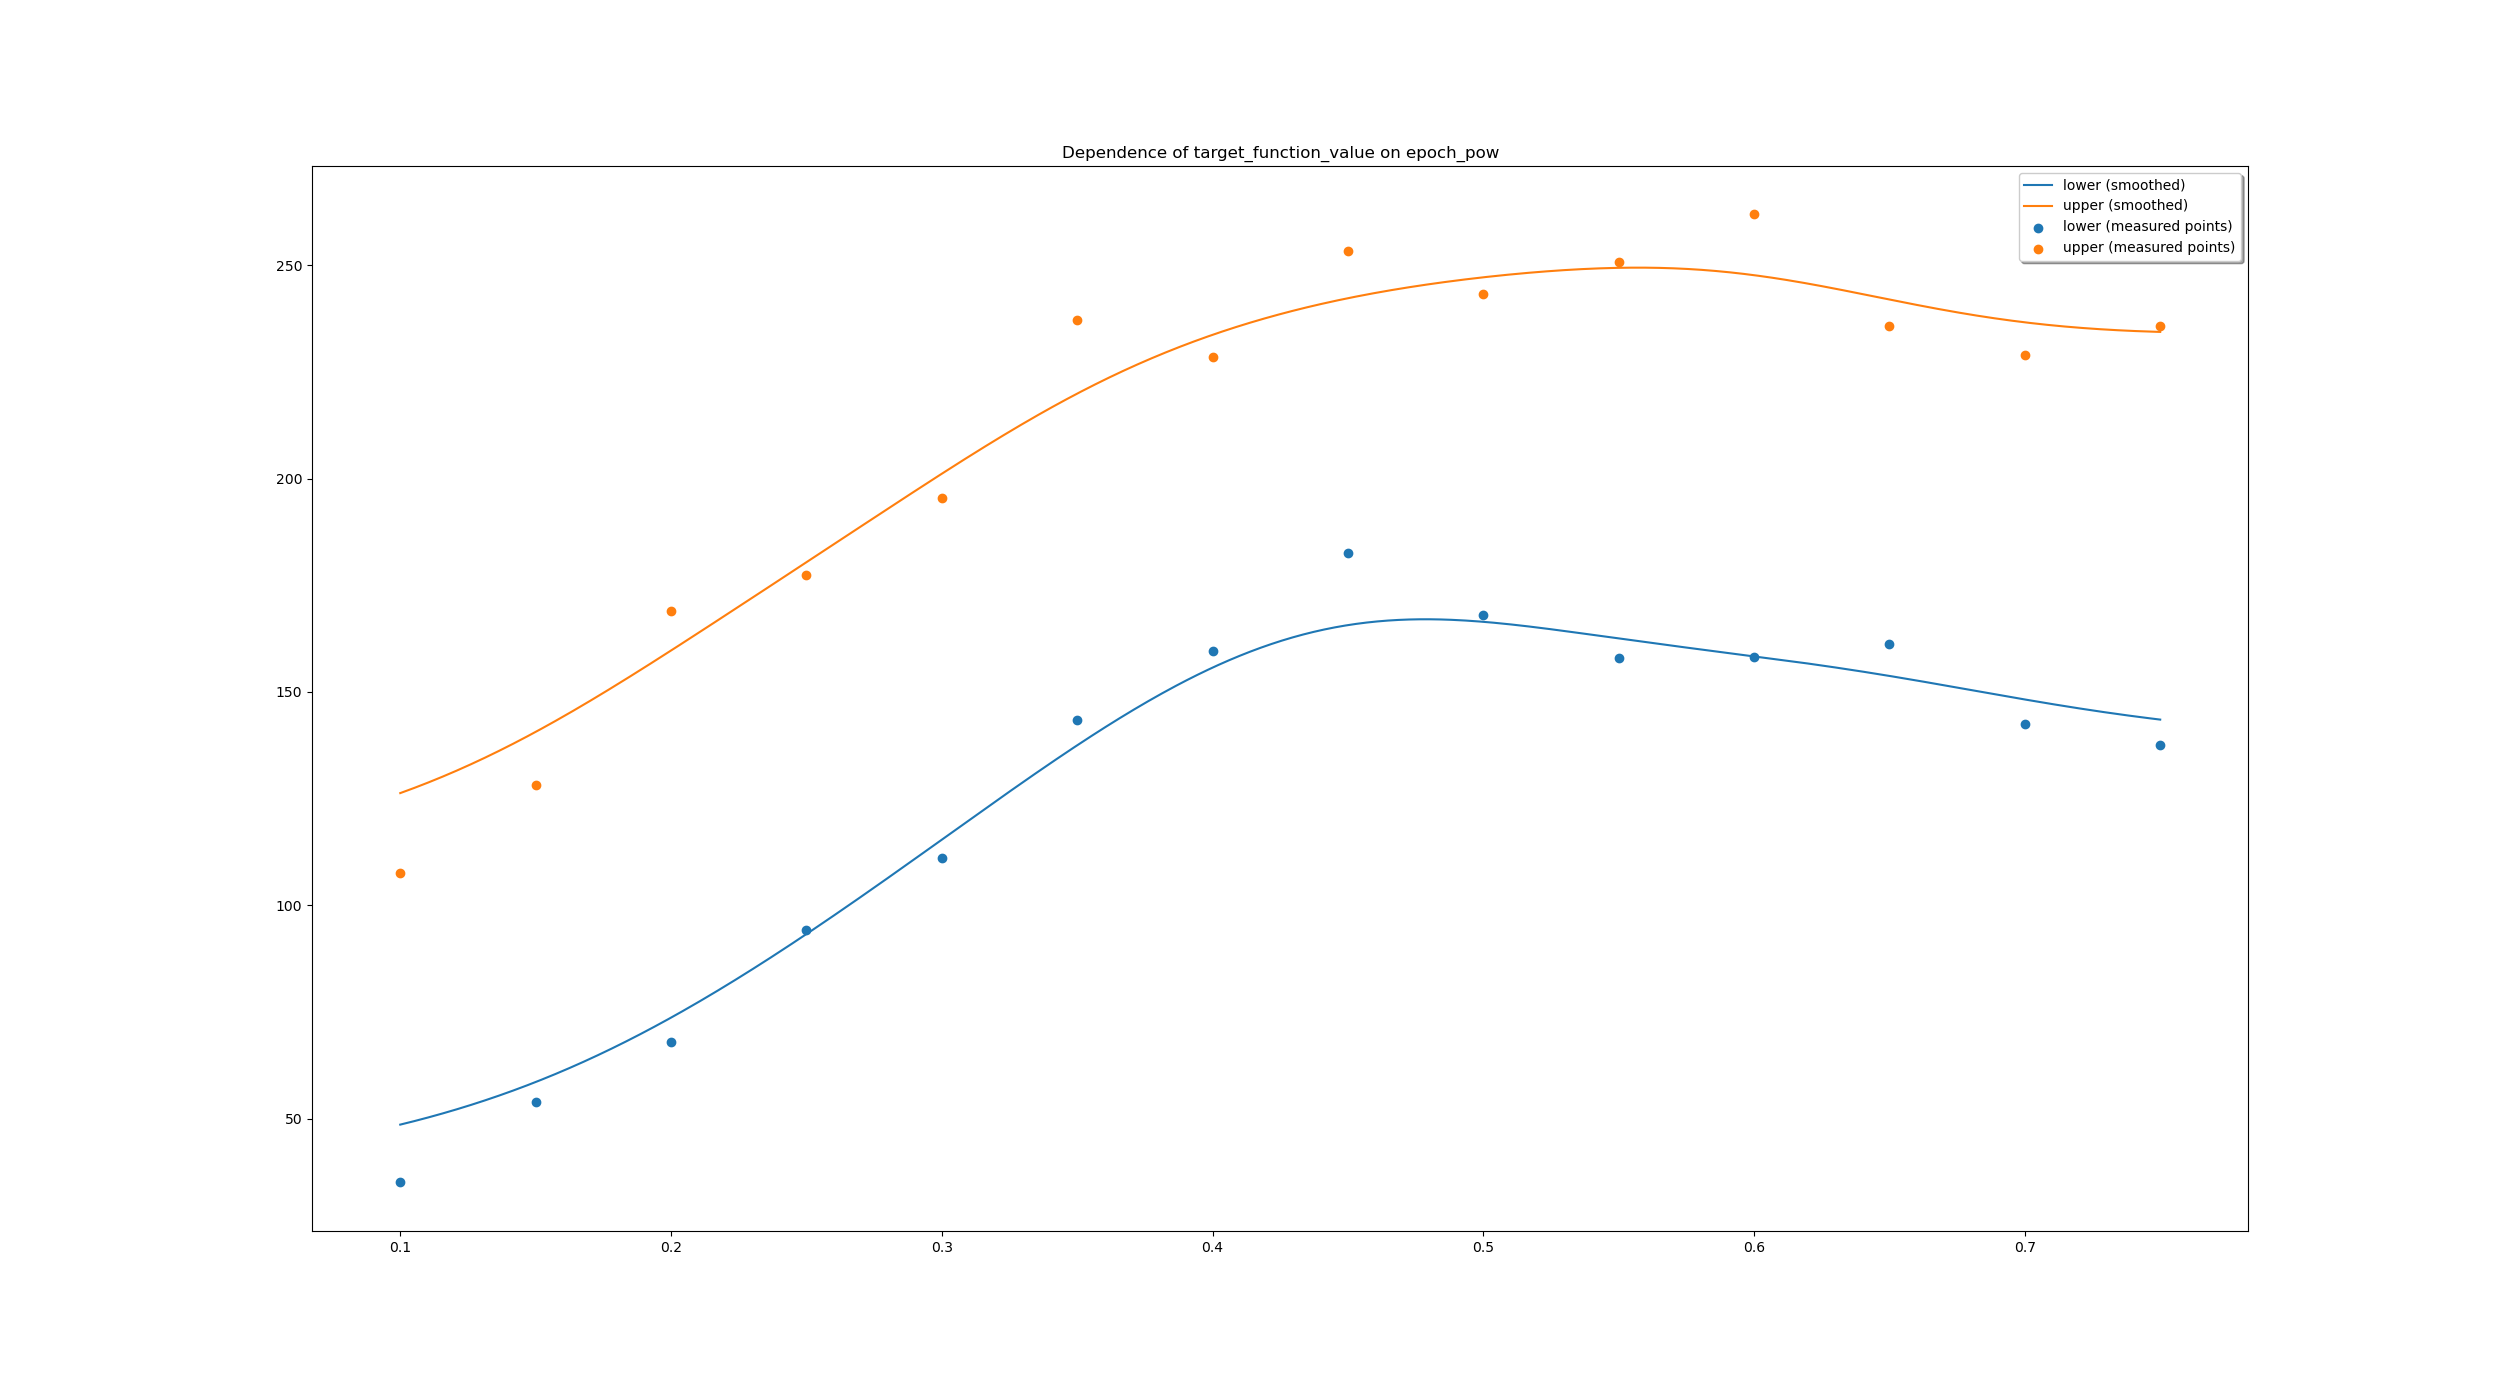
\includegraphics[width=0.75\textwidth]{exploring_optimal_epoch_pow_1000_iterations.png}
        \caption{График для 1'000 вычислений}
        \label{fig:epoch-pow-1000}
    \end{figure}
    \FloatBarrier

    \begin{figure}[h]
        \centering
        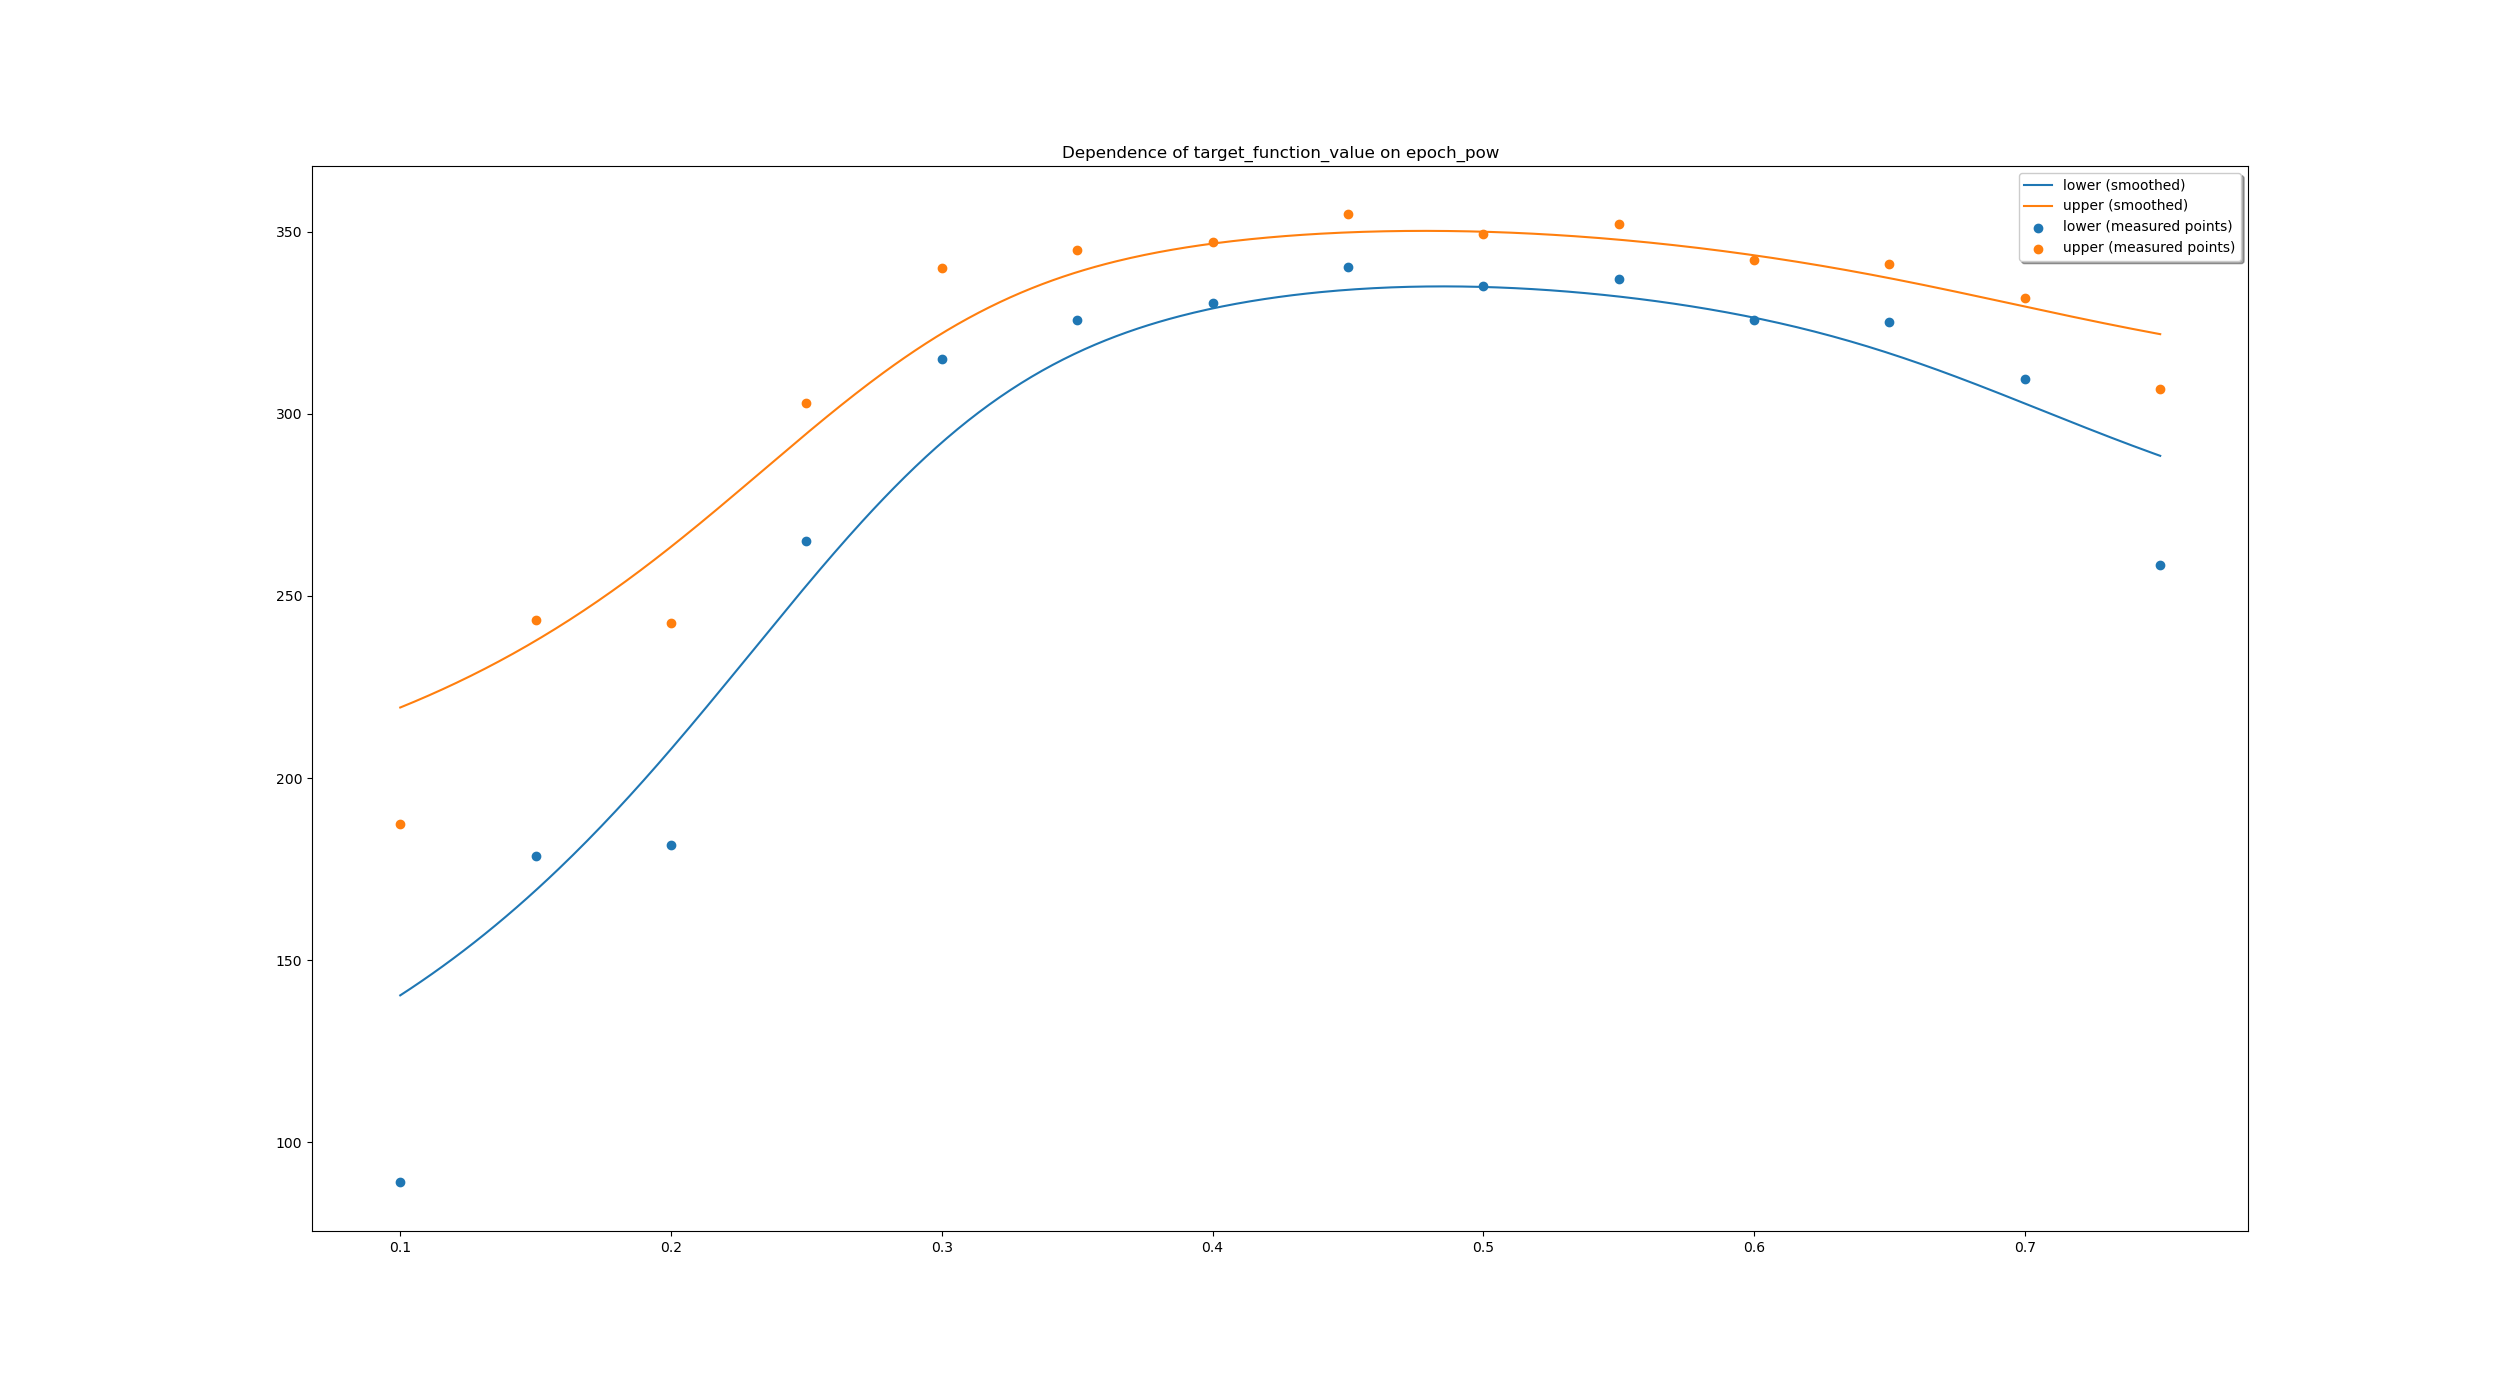
\includegraphics[width=0.75\textwidth]{exploring_optimal_epoch_pow_5000_iterations.png}
        \caption{График для 5'000 вычислений}
        \label{fig:epoch-pow-5000}
    \end{figure}
    \FloatBarrier

    \begin{figure}[h]
        \centering
        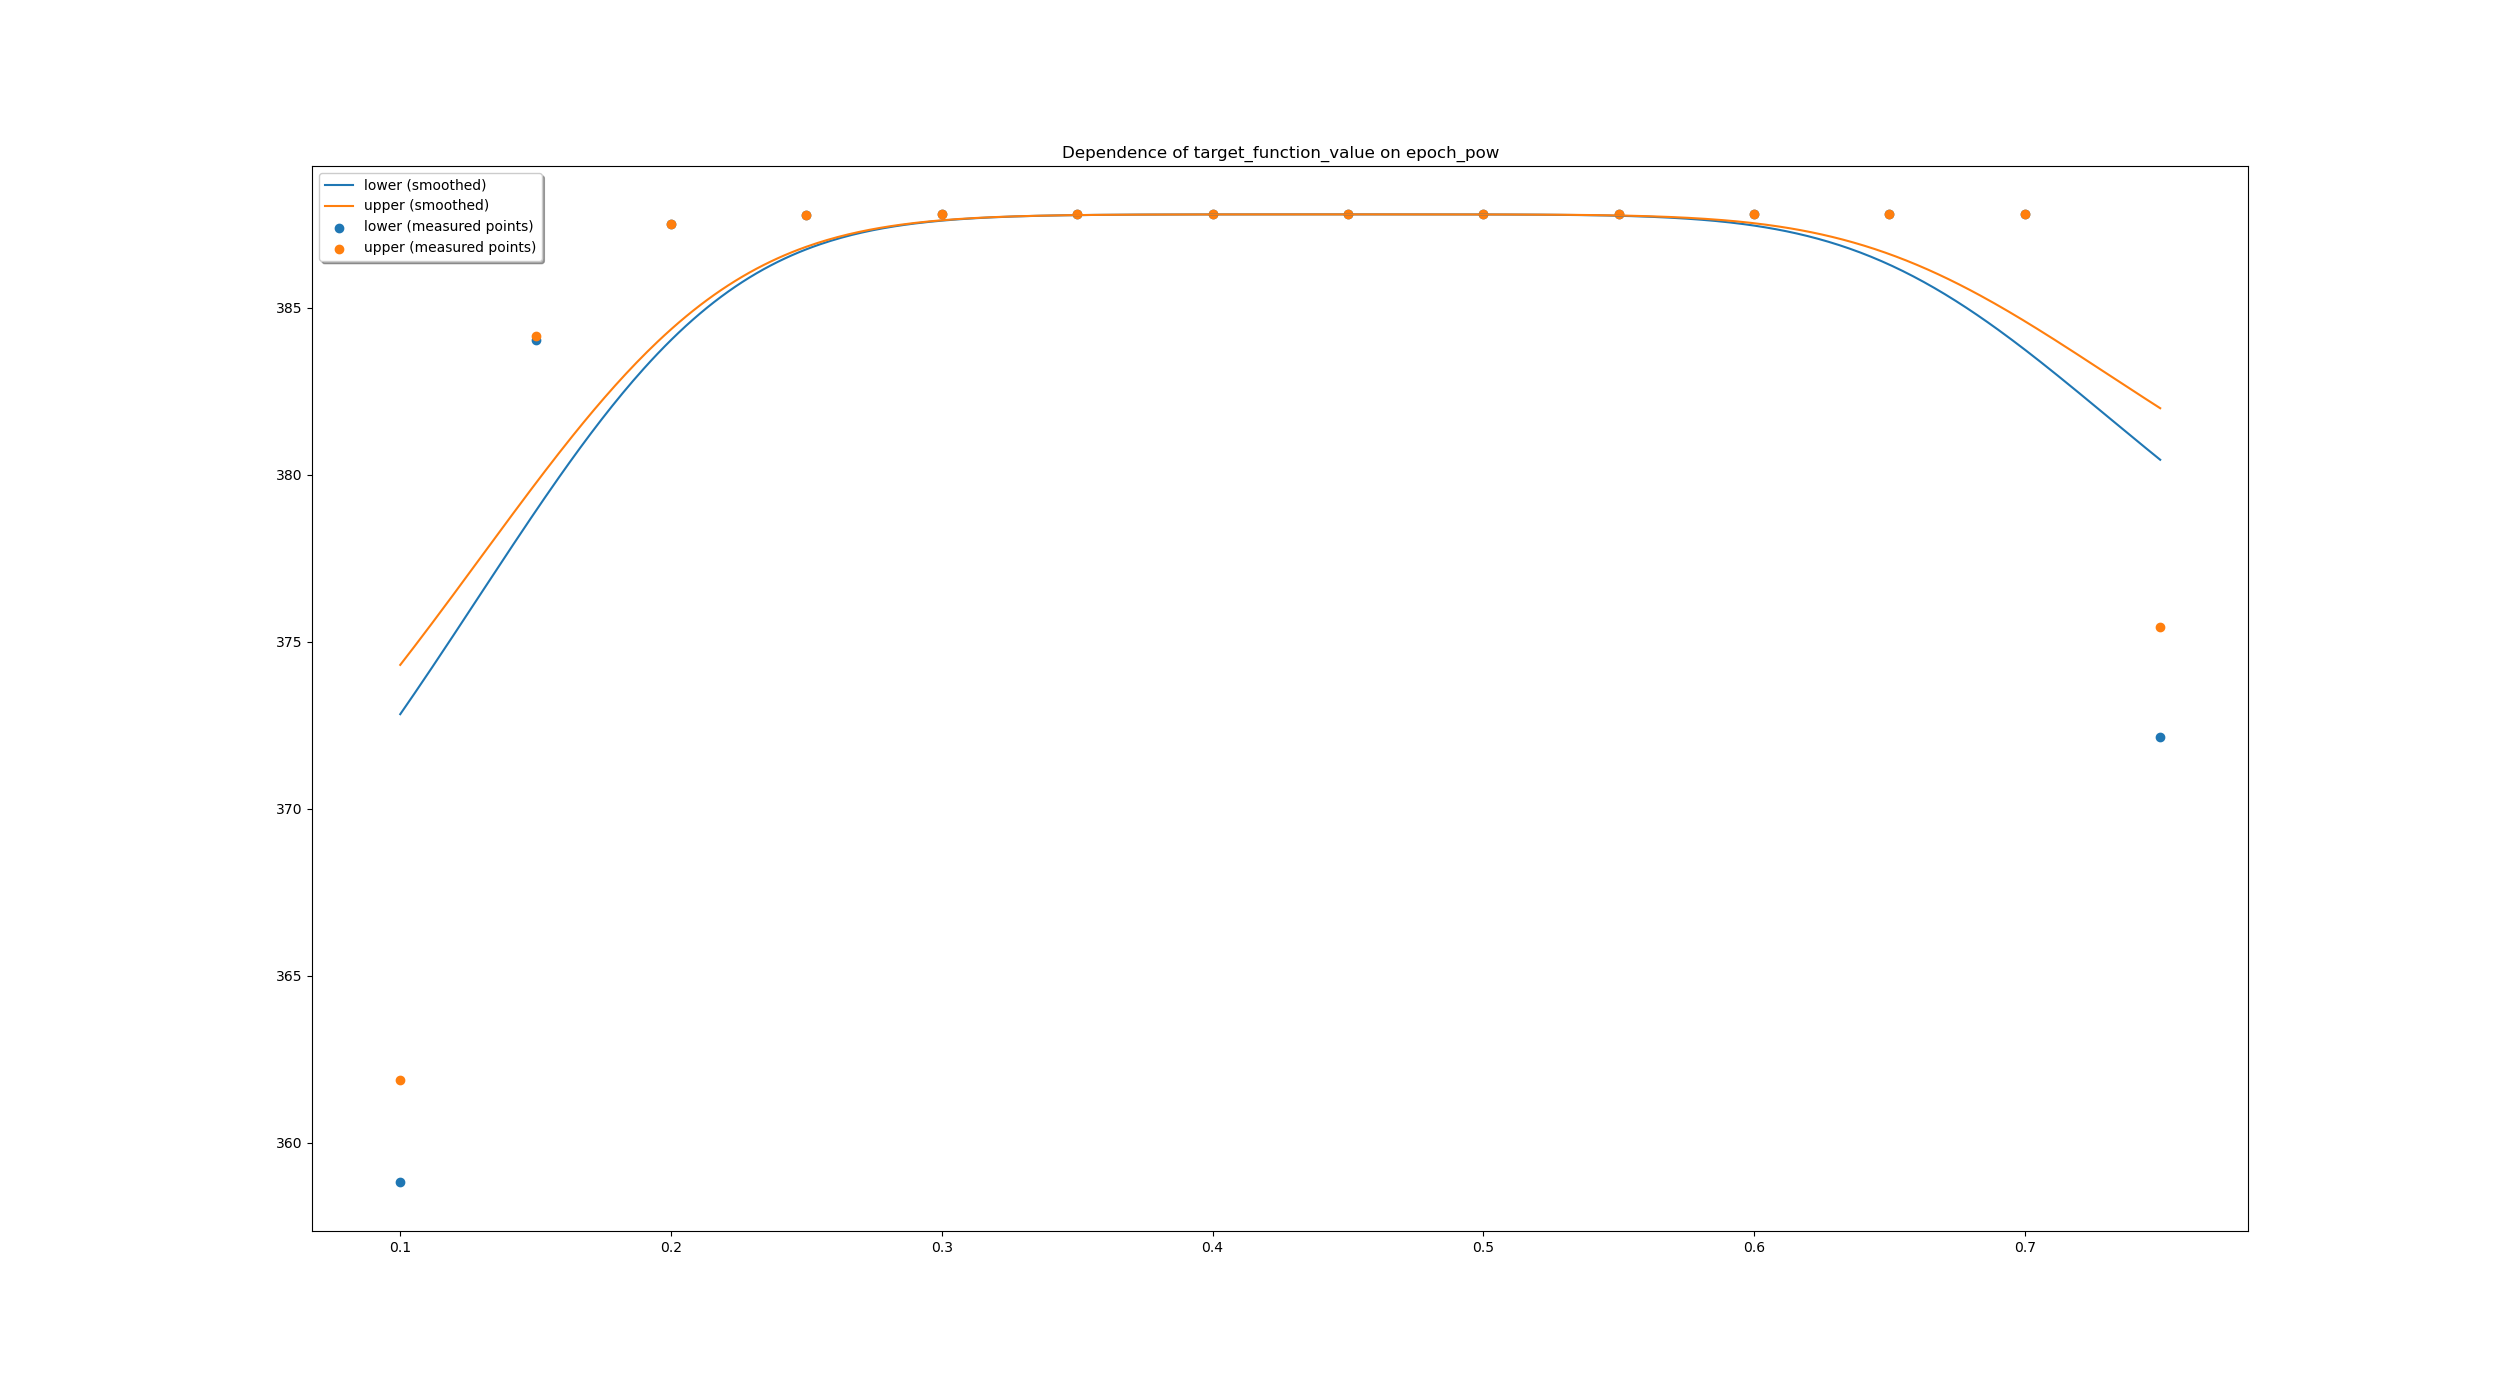
\includegraphics[width=0.75\textwidth]{exploring_optimal_epoch_pow_100000_iterations.png}
        \caption{График для 100'000 итераций}
        \label{fig:epoch-pow-100000}
    \end{figure}
    \FloatBarrier

    Проанализировав полученные данные, я пришёл к выводу, что лучше всего подходит значение $epoch\_pow \approx 0.45$

    \section{Дальнейшее развитие}\label{sec:subsequent-development}
    — Добавить ещё алгоритмы.
    — Использовать аналитические методы, где возможно (например, для решения уравнений)

\end{document}